\graphicspath{{./figures}}

\section{Complete System}
There are various decisions to made with regards to the entire communication system. A complete high-level system block diagram illustrating the decisions discussed below is shown in Figure \ref{fig:complete_system}. Note that the yellow blocks are external, already-provided systems.

\begin{figure}[!htb]
    \centering
    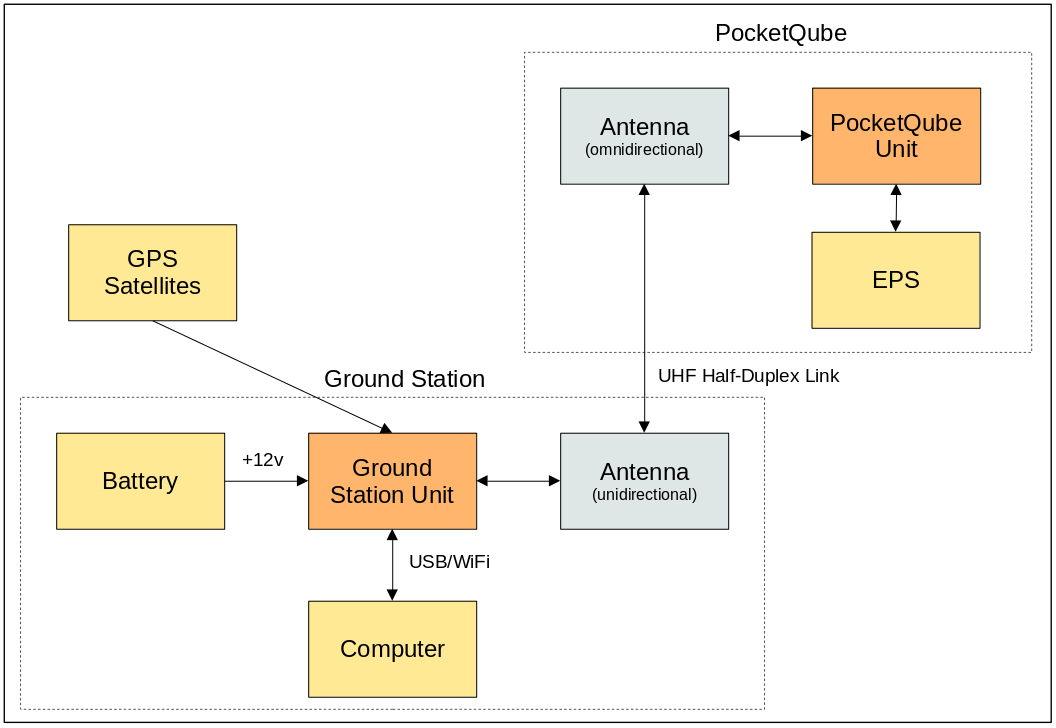
\includegraphics[width=0.8\textwidth]{complete_system.png}
    \caption{Complete High-Level Diagram of Communication System}
    \label{fig:complete_system}
  \end{figure}

Firstly, the requirement to communicate with the existing Radiosonde needs to be taken into account.According to its datasheet \cite{datasheet-iMet54}, it operates at a centre frequency of between 402 and 405 MHz (selected in 1 MHz incremenets). To simplify the design, the custom communication system will use a frequency as close to this as possible, meaning in the UHF band. This will allow for a single ground station antenna to be shared for both systems, at the cost of reduced flexibility of the custom system.

A standard combination of a unidirectional antenna on the ground station, and an omnidirectional antenna on the satellite, will be used. Further, half-duplex communication will be designed for as full-duplex is unnecessary for such a link. This is due to the nature of the link itself i.e. the common command-response pattern used when receiving data from satellites.

A combination of open-loop path-predicted tracking, and radio signal strength tracking, will be used to track the satellite and maintain the link. The ground station therefore requires a GPS connection. The path data will be uploaded to the ground station via USB or WiFi and an external device, such as a laptop, personal computer or smartphone (referred to as the system's \textit{computer} onwards). Further, this computer will be used to monitor the link and record the data.

Finally, the ground station will be powered via +12V from a nearby vehicle, and the PocketQube will be powered from an on-board EPS (another PQ unit). Of course, the sub-systems should be designed such that testing without a vehicle/EPS is possible.